\section{Matematyczne podstawy algorytmów}

\begin{frame}{Puzzle Merkle'a}
    \begin{figure}
        \centering
            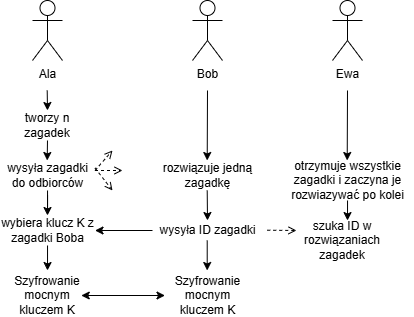
\includegraphics[height=0.45\textwidth]{teoria/graphics/ala_bob_ewa.png}
            \caption{Źródło: własne}
    \end{figure}
\end{frame}

\begin{frame}{Puzzle Merkle'a}
    \begin{center}
    \texttt{15JqVMuLIlyKdkIx} \\
    \texttt{HCzoAJ1ahv8xazFj} \\
    \texttt{9JhU04wO1o6YQ50g} \\
    \texttt{2jVyaS0JLlcKNnC9} \\
    \texttt{...} \\
    \texttt{CZ98NQLvoE9nXph6}
    \end{center}
\end{frame}

\begin{frame}{Puzzle Merkle'a}
    \begin{center}
    \texttt{15JqVMuLIlyKdkIx} \\
    \texttt{HCzoAJ1ahv8xazFj} \\
    \texttt{\textcolor{blue}{9JhU04wO1o6YQ50g}} \\ % Zmiana koloru
    \texttt{2jVyaS0JLlcKNnC9} \\
    \texttt{...} \\
    \texttt{CZ98NQLvoE9nXph6}
    \end{center}
\end{frame}

\begin{frame}{Puzzle Merkle'a}
    \begin{center}
    \texttt{\textcolor{blue}{9JhU04wO1o6YQ50g}} \\
    \pause
    $\Downarrow$ \\
    \texttt{PuzzleID: 17; NewKey: 6nph6LlaqL7YCKsY}
    \end{center}
\end{frame}

\begin{frame}{Puzzle Merkle'a}
    Trudność złamania:
    \begin{center}
        {\Large \( \frac{n \times m}{2} \)} \\[10pt]
    \end{center}
    \( n \) - liczba zagadek \\
    \( m \) - liczba obliczeń potrzebnych do złamania jednej zagadki
\end{frame}